% -*- mode: LaTeX; mode: TeX-PDF; coding: utf-8  -*-


\subsection*{Схема вычислений в модели Open CL}
\label{sec:OCLprog}

%\subsection*{Описание параллельного вычислительного алгоритма  восстановления данных}

%\subsection*{Основные обозначения}
%\subsection*{Описание программы восстановления данных на OCL}

%\emph{OCL реализация алгоритма восстановления данных}
%Выполнена реализация предложенной вычислительной схемы для
%двухмерного случая в стандарте Open CL (Open Computational Language)~\cite{doc_OCL}.

%Выбрана модель массового параллелизма,
%описываемая стандартом Open CL.
%(Open Computational Langua\-ge)~\cite{doc_OCL}.
Open CL является открытым и широко применяемым стандартом для вычислений
общего назначения в 
гетерогенных (неоднородных) системах
(см., например,~\cite{paper_heterog_NIISI, paper_OCL_Komdiv, paper_Deg_Bogd}). 
Одним из известных примеров гетерогенных систем являются системы,
содержащие в своём составе графические процессоры (GPU --- Graphic Processor Unit).
%Современные графические процессоры (GPU --- Graphic Processor Unit)
%включают в себя большое количество простых 
%вычислительных элементов((потом термин!)). %поэтому 
%В силу специфики архитектуры
Такие системы, в силу архитектурной специфики,   
хорошо подходят для эффективной реализации задач,
обладающих массовым параллелизмом.
Вычислительные системы с GPU в настоящее время находят применение не только для
графического рендеринга, но и для %ускорения ((выполнения)) 
эффективного выполнения различного рода
вычислений общего назначения~\cite{}. 

% (известной как GPGPU --- General Purpose GPU).
%В силу специфики архитектуры такие системы 
%хорошо подходят для эффективной реализации задач,
%обладающих массовым параллелизмом.


%% На уровне гетерогенной системы: управляющий процессор -- ускоритель
Модель гетерогенной вычислительной системы в стандарте Open CL 
состоит из управляющего процессора (Host)
и вычислителей (Compute Device),
содержащих, в свою очередь, 
модули (Compute Unit),
которые включают в себя %вычислительные элементы (Processing Element).
рабочие элементы (Work item).
%<Решила использовать вместо вычислительный элемент --- заменить везде!>
Представление вычислительной платформы в Open CL
показано на рисунке~\ref{fig:OCL_platform}.

%<один общий рисунок --- уже сделан отдельно>
\begin{figure}[h!]
  \centering
  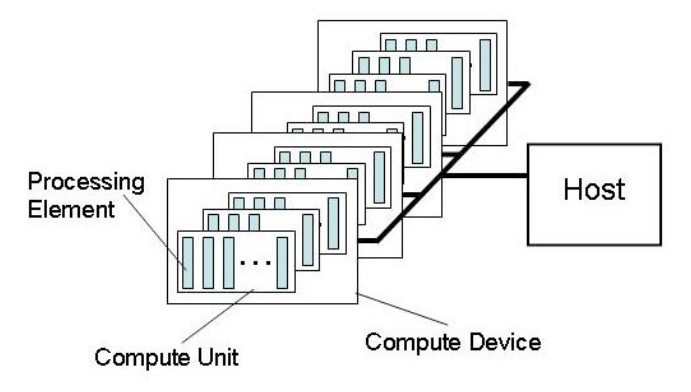
\includegraphics[width=\textwidth,height=7cm]{OCLmodel_platform} 
  \caption{Состав вычислительной платформы в Open CL}
  \label{fig:OCL_platform}
\end{figure}
\FloatBarrier

\begin{figure}[h!]
  \centering
  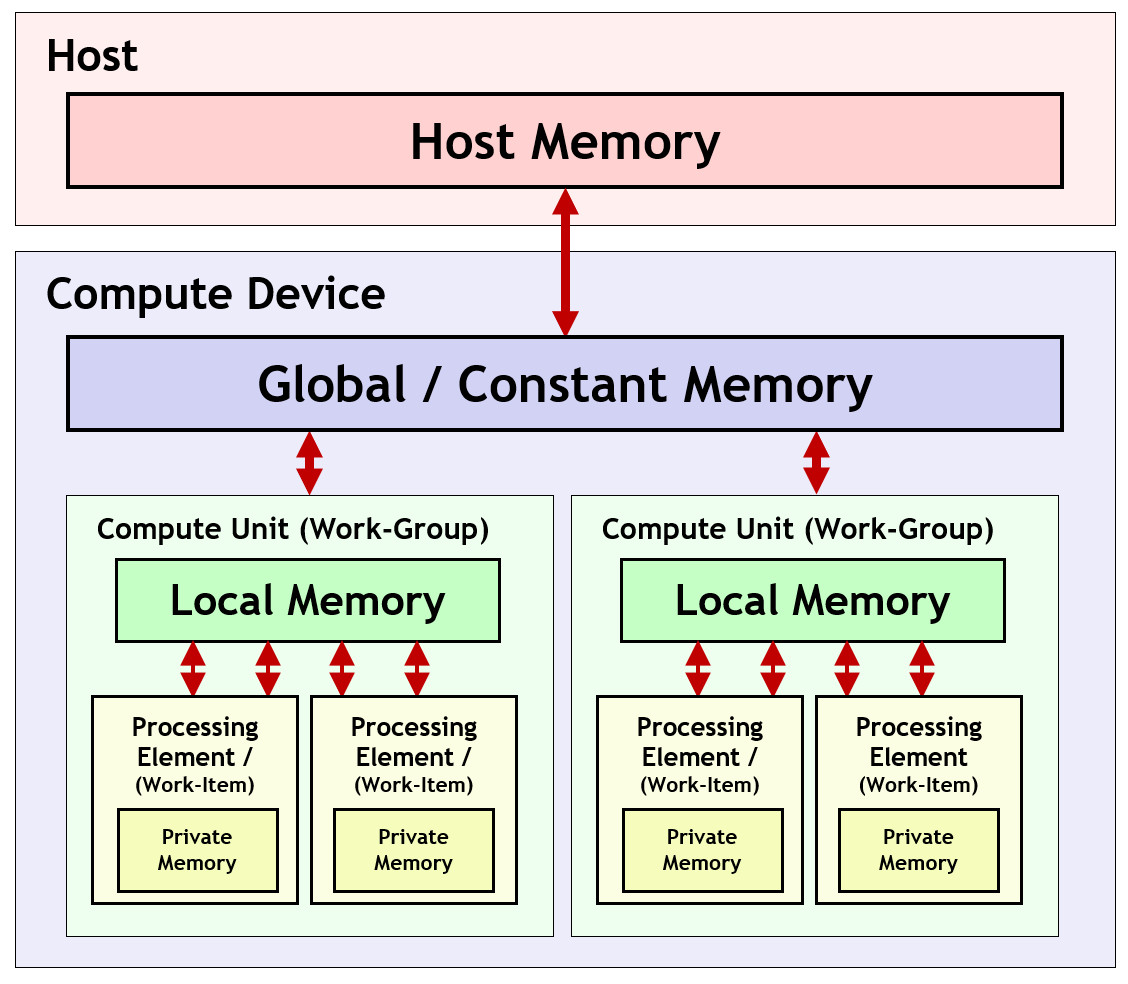
\includegraphics[width=\textwidth,height=7cm]{OCLmodel_mem} 
  \caption{Иерархия памяти вычислительной платформы в Open CL}
  \label{fig:OCLmodel_mem} %{fig:OCL_wg}
\end{figure}
\FloatBarrier




%% Модель памяти
%Иерархия памяти вычислительных ускорителей представляется следующим образом
%Вычислительные устройства
Вычислители
имеют следующую иерархию памяти 
(см. рисунок~\ref{fig:OCLmodel_mem}).
Всем рабочим элементам доступна глобальная память. 
Через глобальную память также происходит обмен данными
с памятью управляющего процессора. 
Каждый модуль 
обладает локальной памятью, к которой имеют доступ
его рабочие элементы.
Каждый рабочий элемент имеют внутреннюю  память (регистры), доступную только ему.

%Execution of an OpenCL program occurs in two parts: kernels that execute on one or more
%OpenCL devices and a host program that executes on the host. The host program defines the
%context for the kernels and manages their execution.
Исполняемая программа, разработанная в стандарте Open~CL,
содержит %:  
вычислительные ядра (kernels), выполняющиеся
параллельно 
в режиме SIMD  
на рабочих элементах  %((ускорителей --- убрать, вообще двусмысленность!))
и управляющую программу, которая
определяет контекст и 
управляет запуском вычислительных ядер.


% ((вместо текста лучше: обобщенная схема разработанного в модели OCL ПО приведена на рисунке))
% ((здесь нет, мне кажется для этой части рисунков достаточно --- возможно рисунок структуры программы
% появится для наших ядер при описании программы))


%% Параллелизм на уровне вычислительных элементов
%Модель параллелизма %программирования
%в OpenCL
%на уровне GPU выражается как SIMT (Single Instruction Multiple Threads) --- терминология CUDA.

%Множество потоков в рамках которых выполняется
%код вычислительных ядер (kernel) выполняется %параллельно
%на множестве вычислительных элементов.

%На уровне абстрации модели вычислений в Open CL ((может как нибудь проще?))
Все рабочие элементы организованы в Open CL в рабочее пространство ---
$n$-мерную решётку,  
размер которой обозначим $NDRange \in \mathbb {N}^n$.
Помимо этого, %((,+))
решётка разбивается на %$n_{wg}$-мерные
рабочие группы, %% отметить кратность!
их размер обозначим $NDWorkGroup \in \mathbb {N}^n$. 

Для каждого рабочего элемента %((в такой -)) модели
определены:  
$GlobalID \in [0: NDRange - \mathbf{1}^n]$ %(в общем случае вектор)
--- индекс вычислительного элемента; %из $[0: NDRange - \mathbf{1}^n]$;
%в пространстве размерности задачи (NDRange).
$LocalID \in [0: NDWorkGroup - \mathbf{1}^n]$ ---
индекс вычислительного элемента в рабочей группе.
%из $[0: NDWorkGroup - \mathbf{1}^n]$. 
%пространстве размерности рабочей группы (Work Group).
На рисунке~\ref{fig:OCL_wg} приведён пример
часто встречающегося на практике двумерного рабочего пространства.

<будет переделан>
\begin{figure}[h!]
  \centering
  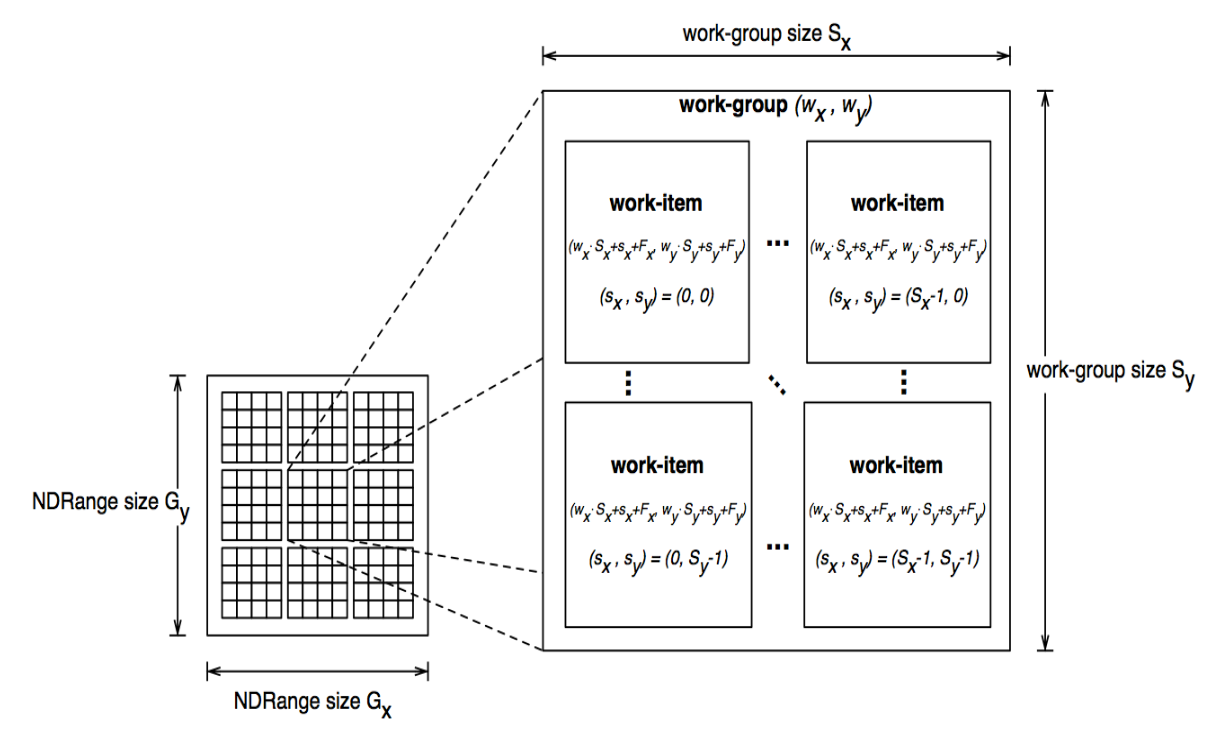
\includegraphics[width=\textwidth,height=7cm]{OCLmodel_wg} 
  \caption{Пример модели рабочего пространства Open CL}
  \label{fig:OCL_wg}
\end{figure}
\FloatBarrier


%%% Local Variables: 
%%% mode: latex
%%% TeX-master: "paper_func_recv"
%%% End: 



